\documentclass{SeminarV2}

\usepackage[latin1]{inputenc}
\usepackage{amssymb,amsmath,array}
\usepackage{graphicx}
\usepackage{placeins}


%***********************************************************************
% !!!! IMPORTANT NOTICE ON TEXT MARGINS !!!!!
%***********************************************************************
%
% Please avoid using DVI2PDF or PS2PDF converters: some undesired
% shifting/scaling may occur when using these programs
% It is strongly recommended to use the DVIPS converters.
%
% Check that you have set the paper size to A4 (and NOT to letter) in your
% dvi2ps converter, in Adobe Acrobat if you use it, and in any printer driver
% that you could use.  You also have to disable the 'scale to fit paper' option
% of your printer driver.
%
% In any case, please check carefully that the final size of the top and
% bottom margins is 5.2 cm and of the left and right margins is 4.4 cm.
% It is your responsibility to verify this important requirement.  If these margin requirements and not fulfilled at the end of your file generation process, please use the following commands to correct them.  Otherwise, please do not modify these commands.
%
\voffset 0 cm \hoffset 0 cm \addtolength{\textwidth}{0cm}
\addtolength{\textheight}{0cm}\addtolength{\leftmargin}{0cm}

%***********************************************************************
% !!!! USE OF THE SeminarV2 LaTeX STYLE FILE !!!!!
%***********************************************************************
%
% Some commands are inserted in the following .tex example file.  Therefore to
% set up your Seminar submission, please use this file and modify it to insert
% your text, rather than staring from a blank .tex file.  In this way, you will
% have the commands inserted in the right place.

% Edited by Martin Bogdan.

\begin{document}
%style file for Seminar manuscripts
\title{User Manual}

%***********************************************************************
% AUTHORS INFORMATION AREA
%***********************************************************************
\author{Maximilian Joas$^1$
%
% Optional short acknowledgment: remove next line if non-needed
%\thanks{This is an optional funding source acknowledgement.}
%
% DO NOT MODIFY THE FOLLOWING '\vspace' ARGUMENT
\vspace{.3cm}\\
%
% Addresses and institutions (remove "1- " in case of a single institution)
University of Leipzig  - Department of Computer Science \\
Augustusplatz 10, 04109 Leipzig  - Germany\\}

%
% Remove the next three lines in case of a single institution

%***********************************************************************
% END OF AUTHORS INFORMATION AREA
%***********************************************************************

\maketitle

\begin{abstract}


\end{abstract}

\section{multiVitamin}
mulitVitamin is a software package to perform mulitple alignments with graphs.
There are two algorithmns availbale for this task. The Bron Kerbosch \cite{}
and the VF2 algorithmn \cite{}. Details on the algorithmns ca be found in the
theory section.\\
The main function of the package is to allign two or more graphs. This results
in a Newick Tree of the best allignment. and the resulting multiple alignent, which
is represented as a graph.
\cite{}  Sounds exciting, so let's
get started and show how to use this baby.
\section{Installation}

Clone the repo from github with: \\
%git clone https://github.com/MaxJoas/graph_alignment.git
Navigate in the directory where the setup.py file is: \\
%cd multivitamin_project/multivitamin/multivitamin
install with pip3 install -e .
Done now you can use multiVitamin as a command.



\section{Graph Format}

A good first step is to famliarize yourself with the graph format. A graph
file is basically a .txt file, we use the .graph to be more specific.
Every graph consists of nodes and edges. Every node as an id, which is an unique
integer for each node. Optionally nodes can be labelled. The id and label are
seperated by a semicolon. The edges are two connected nodes and represented
by the ids of the two nodes seperated with a semicolon.\\
The file itself is structered as follows: \\
The first line indicates the authors of the graph. The second line shows the number
of node and the third line the number of edges
This is followed by three lines
that indicate whether the nodes / edges are labelled and if the graph is directed.
A blank line indicates the start of the node section, which are represented as
descirbed above. The node section is followed again by a blank line and the edge section.
Let's look at a small example graph for illustration. The graph has 6 nodes
which are all labelled with a 'c' and 6 edged which are not labelled.
Your graphs need to have exactely this format to use this package. expecially
the blank lines are important. For further example graphs go to the root
directory and navigate to the graphs directory. Now that you are familiar with
the graph format, we can take a look how to use the package.
\begin{verbatim}
AUTHOR: Michel K.
#nodes;6
#edges;6
Nodes labelled;True
Edges labelled;False
Directed graph;False

1;c
2;c
3;c
4;c
5;c
6;c

1;2
1;6
2;3
3;4
4;5
5;6
\end{verbatim}

\section{Graph Alignment}
Consider the basic use without any options for the start.
You do not have to be in the directory of the package to use mulitVitamin.
Just type "mulitVitamin -f <pathToGraphFile1.graph> <pathToGraphFile2> <optionalMoreGraphFiles>"
in the command line. This aligns the given graphs with the Bron Kerbosch algorithmn.
The resulting command line seems confusing at first put follows a clear structure
and provides all the important information about the alignment."
in the command line. This aligns the given graphs with the Bron Kerbosch algorithmn.
The resulting command line seems confusing at first put follows a clear structure
and provides all the important information about the alignment.
In order to see from which graph each node of the alignent origins, we use
abbrevations of the names of the graph input files. A dictionary of the abbrevations
of the original names of the graph files is shown first in the command line output.
The you see the nodes of the alignment. Each line corresponds to one node
of the alignment. A node in an alignment is represented by all nodes that got mathed
to eachother. The aligned node is represented as follows:
The id of th enode consits of the graph id (more specific of the abbrevation of the graph id) of the
graph where the node origins from. This is followed by a dot, followed by the id
of the original node. after a space comes the next aligned node. After all the
id follows a tab and the label of the aligned node (if the graphs were labelled).
After another tab the neighbors of the node are listed. The next line shows
the same for the next node of the alignment.\\
The next section shows the edges of the aligned graph. The format follows the format
of the edges. It basically shows to nodes seperated by a comma and a tab. \\


\begin{figure}[h]
     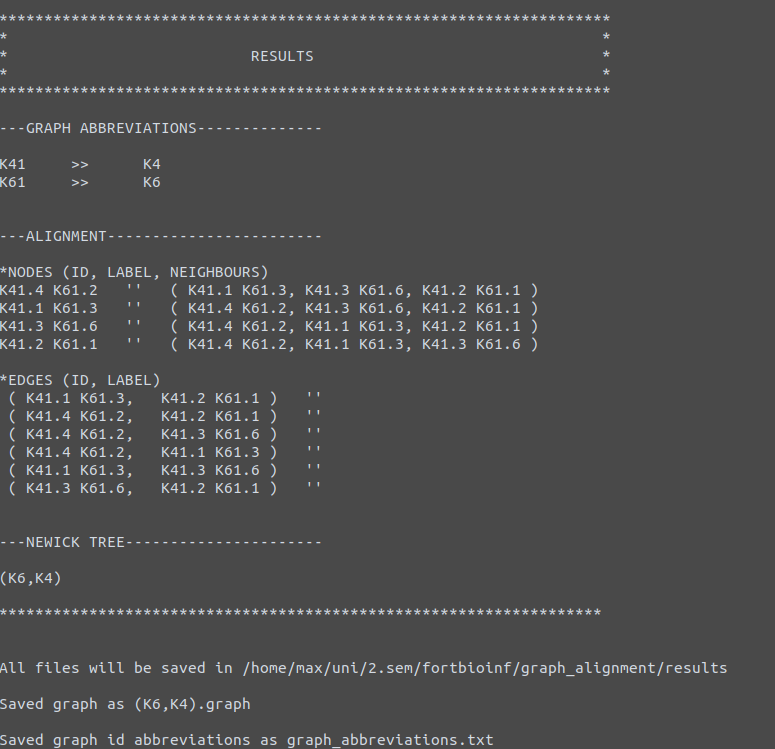
\includegraphics[width=0.5\textwidth]{mulitOut.png}}
  \caption{A picture of the same gull
           looking the other way!}
\end{figure}









% ****************************************************************************
% BIBLIOGRAPHY AREA
% ****************************************************************************

\begin{footnotesize}
\bibliography{own.bib}
\bibliographystyle{unsrt}
% IF YOU DO NOT USE BIBTEX, USE THE FOLLOWING SAMPLE SCHEME FOR THE REFERENCES
% ----------------------------------------------------------------------------

% ----------------------------------------------------------------------------

% IF YOU USE BIBTEX,
% - DELETE THE TEXT BETWEEN THE TWO ABOVE DASHED LINES
% - UNCOMMENT THE NEXT TWO LINES AND REPLACE 'Name_Of_Your_BibFile'


%\bibliography{Name_Of_Your_BibFile}

\end{footnotesize}

% ****************************************************************************
% END OF BIBLIOGRAPHY AREA
% ****************************************************************************

j\end{document}
